\documentclass{article}
\usepackage[utf8]{inputenc}








\font\myfont=cmr12 at 30pt
\title{\myfont EE568 Project 3 - PM Motor Comparison Analysis }
\font\hisfont=cmr12 at 20pt
\author{\hisfont by Hakan Saraç - 2408086}
\date{}



\usepackage{natbib}
\usepackage{graphicx}
\usepackage{indentfirst}
\usepackage{siunitx}
\usepackage{svg}
\usepackage{hyperref}
\usepackage{amsmath, bm}
\usepackage{graphicx} 
\usepackage{pstool}

\addtolength{\oddsidemargin}{-.875in}
\addtolength{\evensidemargin}{-.875in}
\addtolength{\textwidth}{1.75in}
\addtolength{\topmargin}{-.875in}
\addtolength{\textheight}{1.75in}    
\begin{document}

\maketitle

\newpage

\tableofcontents
\newpage

\section*{Introduction}
In this project, machines with different constraints will be designed and analyzed. The first constraint is to have a fixed inner diameter. Later, the constraint is updated as a fixed stator outer diameter and new machine is designed. 


Following that, the fixed stator outer diameter machine is compared for different rotor permanent magnets. An optimized neodymium magnet is first designed and compared with a optimized ferrite machine in terms of inner diameter, cost etc.
\section{Question 1 - Magnetic Loading}
\subsection{Part - a}

Flux path for one pole pair is provided in Figure \ref{fig:FluxPath} and the corresponding equivalent magnetic circuit is provided in Figure \ref{fig:MagneticCircuit}. In this part, the permeability of the rotor and stator are assumed to be infinite. Therefore, the reluctance of core material becomes zero. Another assumption can be made as that there is no fringing or leakage flux and flux lines are straight as shown in Figure \ref{fig:FluxPath} with green lines. \newline
The machine parameters are as follows:
\begin{itemize}
    \item Number Of Poles: 4
    \item Motor Axial Length: 100 mm
    \item Air Gap Clearance: 1 mm
    \item Magnet To Pole Pitch Ratio: 0.8
    \item Rotor Diameter: 100 mm
    \item Magnet Thickness: 4 mm
    \item Magnet Type: NdFeB N42 grade (ur=1.05), radial shaped
\end{itemize} 
\bigskip
\noindent With the assumptions made, the reluctance $R_{m1}$ and $R_{m2}$ in Figure \ref{fig:FluxPath} can be calculated as:

\begin{equation} \label{eqn:PoleAreaFormula}
    A_{pole} = \frac{\pi \: D_i \: L_{axial}}{N_{pole}}=0.007853 \: \mathrm{m^2}
\end{equation}
where P is the number of poles.

\bigskip


\noindent From the magnet to pole pitch ratio value of 0.8 (shown as $K$ in (\ref{eqn:MagnetAreaPerPole})), the magnet area per pole can be calculated. 
\bigskip

\begin{equation} \label{eqn:MagnetAreaPerPole}
    A_{magnetperpole} = A_{pole}\cdot K = 0.006283 \: \mathrm{m^2}
\end{equation}

\begin{equation} \label{eqn:NonMagnetAreaPerPole}
    A_{nonmagnetperpole} = (1-K) \cdot A_{pole} = 0.00157 \: \mathrm{m^2}
\end{equation}

\begin{equation} \label{eqn:MagnetReluctance}
    R_{m1}  =  R_{m2} =  \frac{H_{magnet}}{A_{magnetperpole} \cdot \mu_0 \cdot \mu_r}  = 482480 \: \mathrm{\frac{1}{Henry}} 
\end{equation}

\begin{equation} \label{eqn:AirGapReluctance}
    R_{ag1}  =  R_{ag2} =  \frac{H_{airgap}}{A_{magnetperpole} \cdot \mu_0}  =  126650  \: \mathrm{\frac{1}{Henry}} 
\end{equation}

\begin{equation} \label{eqn:MmfPerMagnet}
    \mathcal{F}_{permagnet} = A_{magnetperpole} \cdot B_{residual} \cdot R_{m1} = 4001.61 \: \mathrm{Amperes}
\end{equation}

\bigskip

\noindent Assuming that the core is infinitely permeable, loop equation of the equivalent circuit (see Fig.\ref{fig:MagneticCircuit}) results in (\ref{eqn:AirGapFlux}).
\bigskip

\begin{equation} \label{eqn:AirGapFlux}
    \phi_{m} = \frac{2 \cdot \mathcal{F}_{permagnet}}{R_{m1}+R_{m2}+R_{ag1}+R_{ag2}} = 6.57 \: \mathrm{mWeber}
\end{equation}

\begin{equation} \label{eqn:AirGapFluxDensity}
    B_{m} = \frac{\phi_{m}}{A_{magnetperpole}} = 1.0455 \: \mathrm{Tesla}
\end{equation}
However, the FEA simulations gave a peak flux density value of $1.0174\: \mathrm{T} $ while the analytical calculations are $ 1.0455  \: \mathrm{T}$. The difference is due to the leakage flux. 

\noindent From the values found in (\ref{eqn:AirGapFluxDensity}), the magnetic field strength value is provided in (\ref{eqn:MagneticFieldStrength}).
\begin{equation} \label{eqn:MagneticFieldStrength}
    H_m = \frac{B_m-B_{residual}}{\mu_r \cdot \mu_0} = -208004.48 \: \mathrm{\frac{A}{m}}
\end{equation}

As stated  \href{https://e-magnetsuk.com/neodymium_magnets/neodymium_grades.aspx}{in this website}., the coercivity value for a N42 NdFeB magnet is around $\pmb{955} \: \pmb{\mathrm{\frac{kA}{m}}}$. The load line of the magnets are provided in Fig.\ref{fig:BHCurve}.

\subsection{Part - b}
The magnetic loading of the machine is given in (\ref{eqn:MagneticLoading})
\begin{equation} \label{eqn:MagneticLoading}
    \bar{B} = \frac{N_{pole}\:\phi_{m}}{\pi \: D_i \: L_{axial}} = 0.8364 \: \mathrm{Tesla}
\end{equation}

\subsection{Part - c}
The FEA results are provided in Figure \ref{fig:MagB}.
\begin{figure}[h!]
\centering
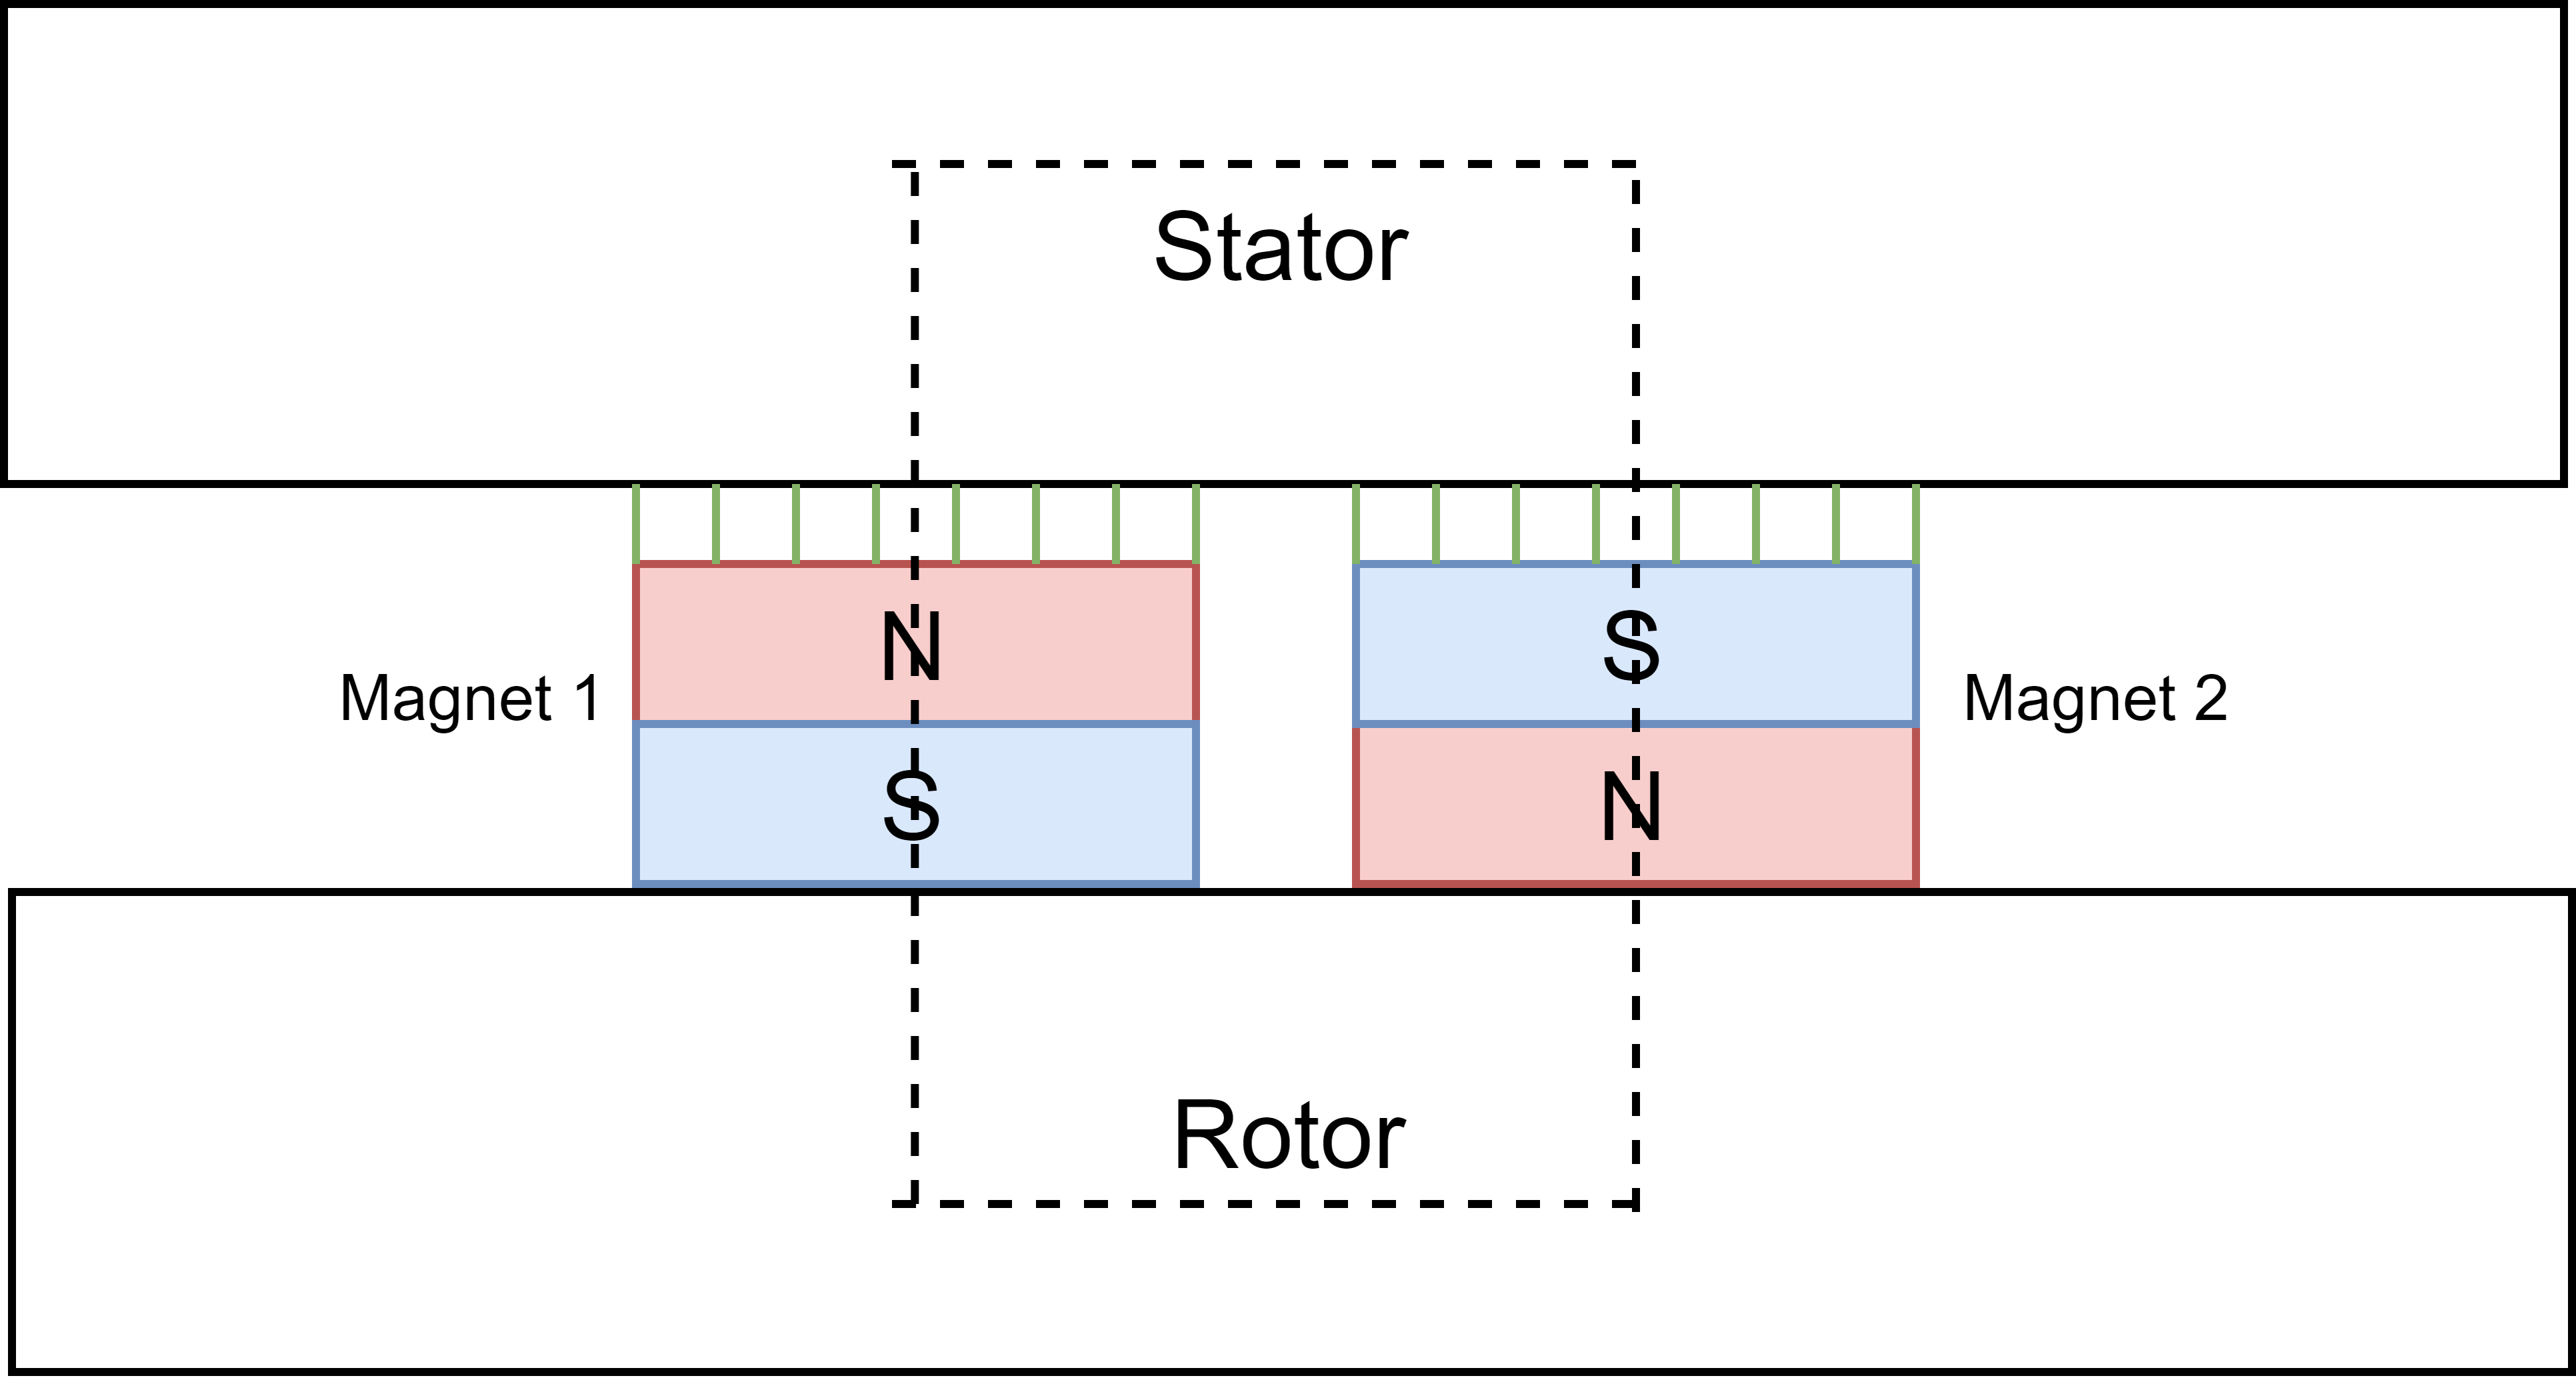
\includegraphics[scale=1.2]{Figures/FluxPath.png}
\caption{Flux Path Through a Pole Pair }
\label{fig:FluxPath}
\end{figure}


\begin{figure}[h!]
\centering
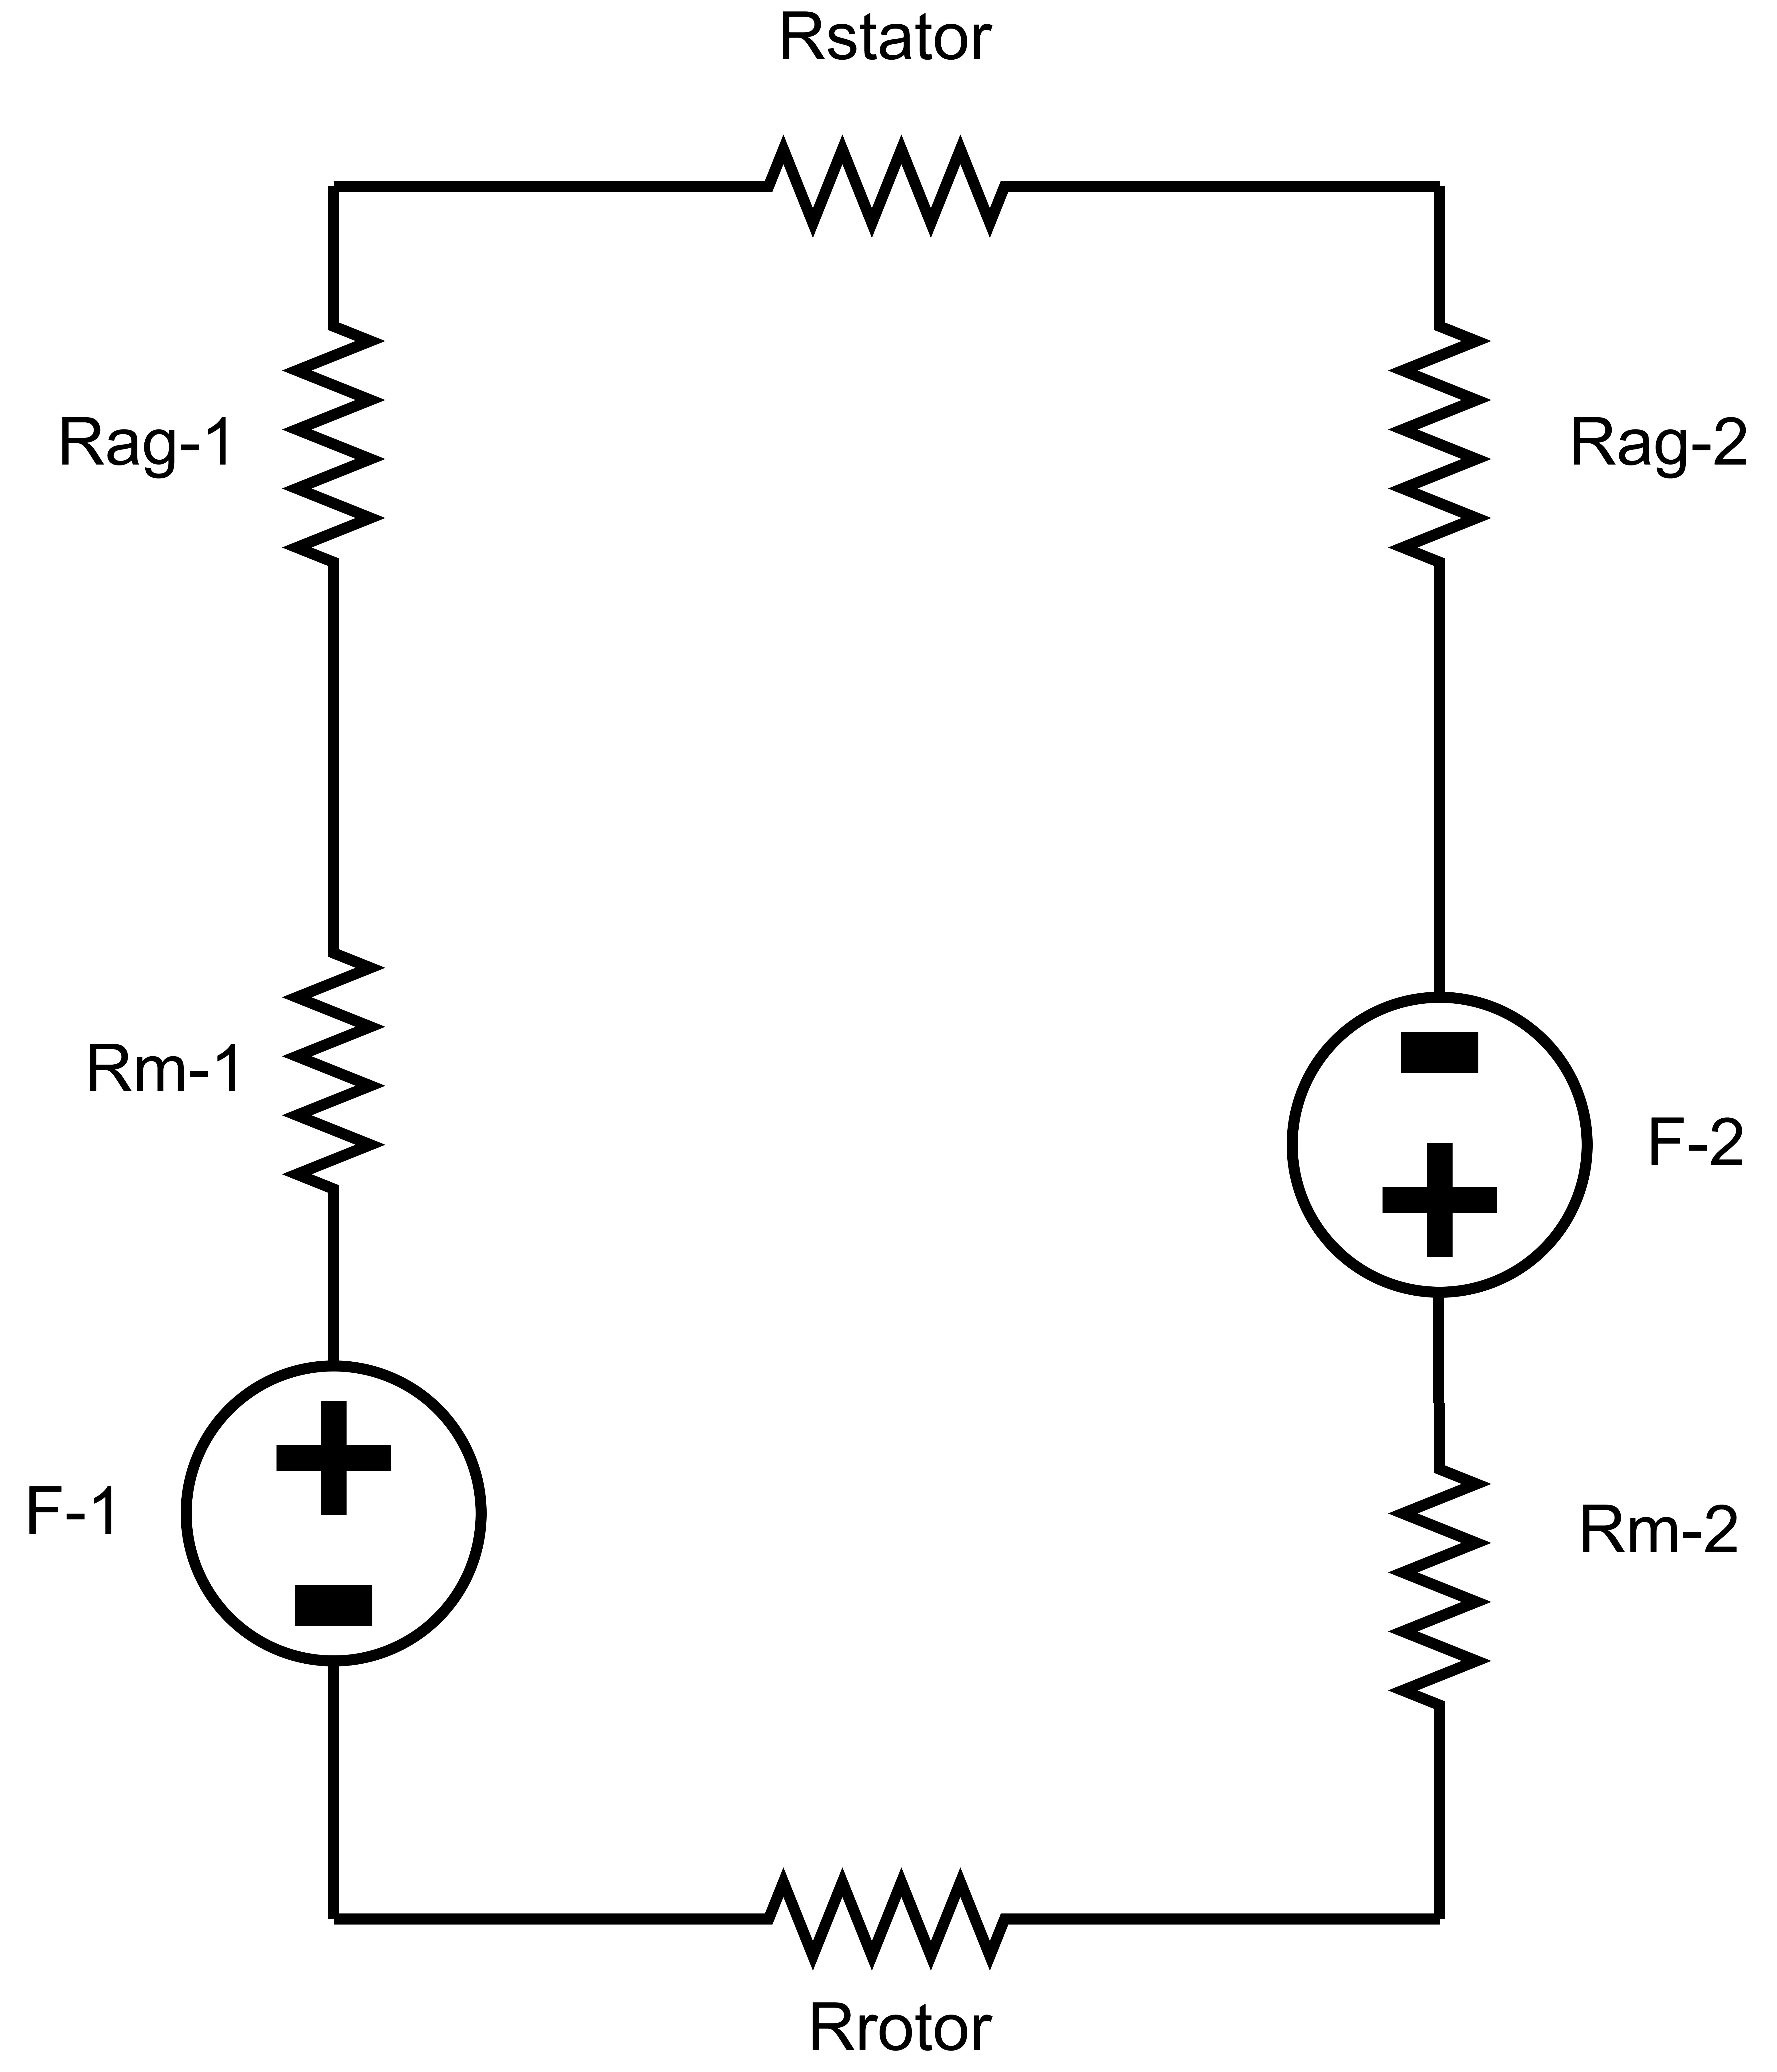
\includegraphics[scale=0.5]{Figures/MagneticCircuit.png}
\caption{Magnetic Equivalent Circuit }
\label{fig:MagneticCircuit}
\end{figure}
\begin{figure}[h!]
\centering
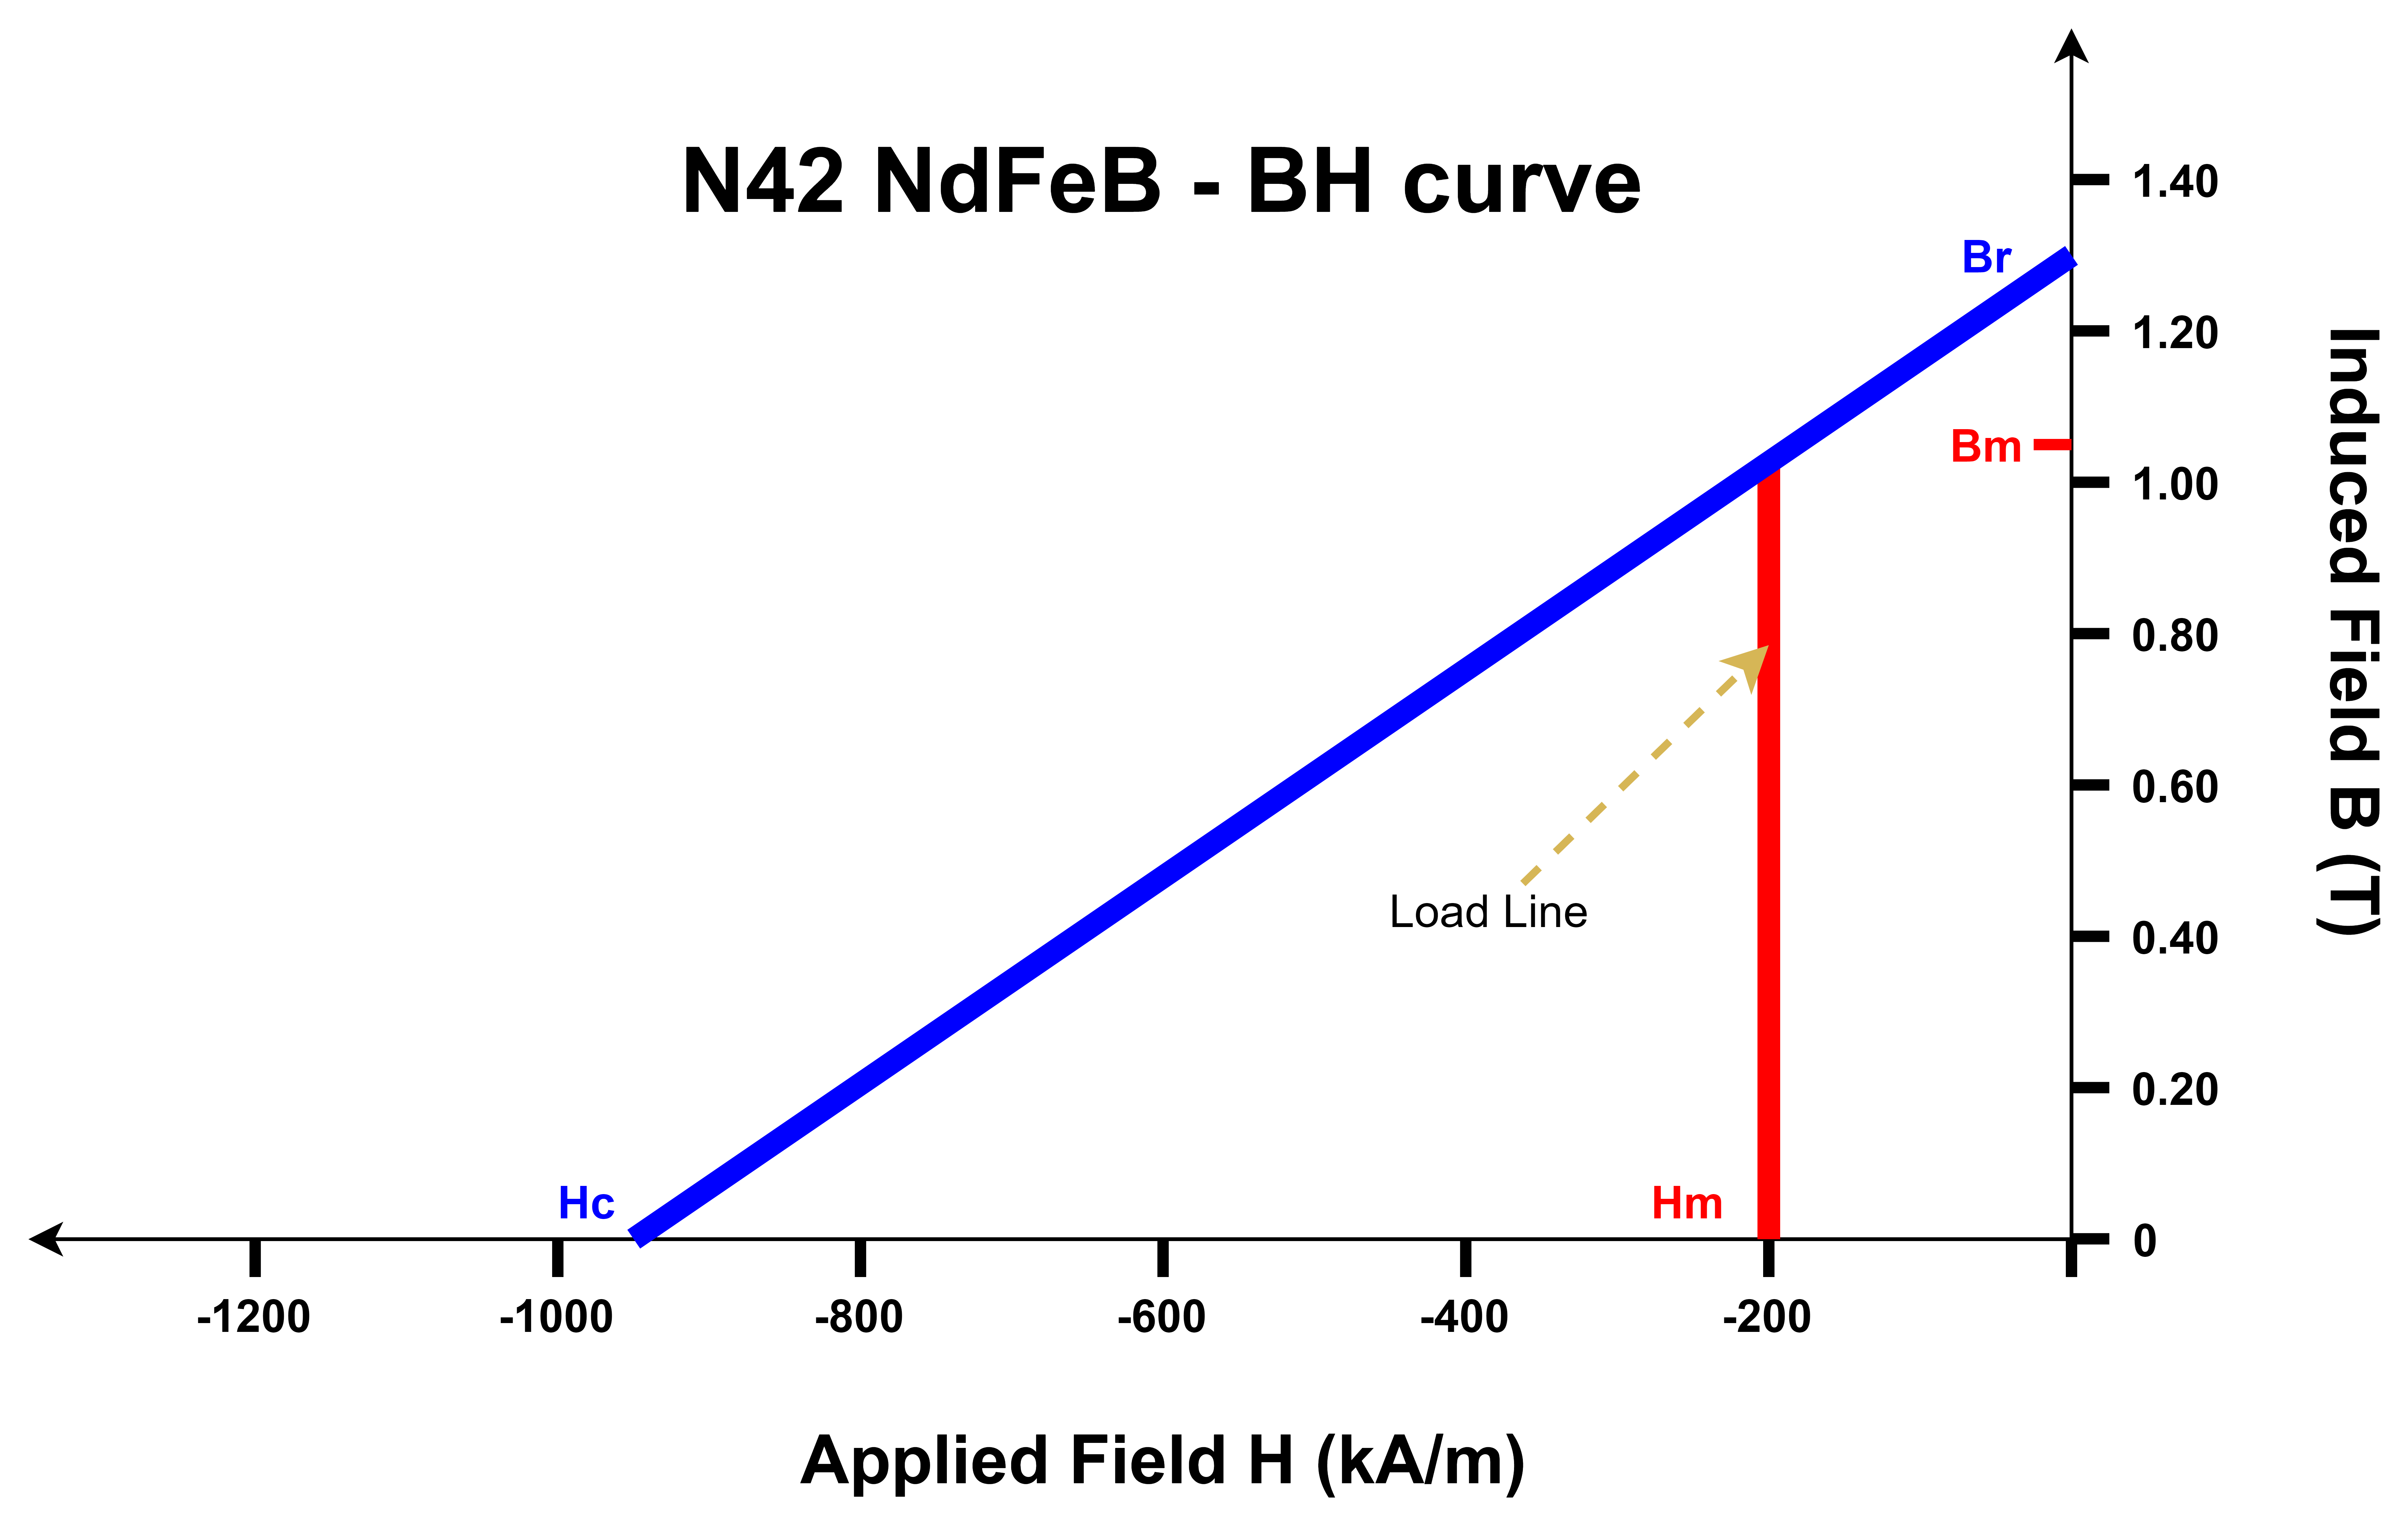
\includegraphics[scale=0.8]{Figures/BHCurve.png}
\caption{N42 NdFeB - BH curve with load line}
\label{fig:BHCurve}
\end{figure}

\begin{figure}[h!]
\centering
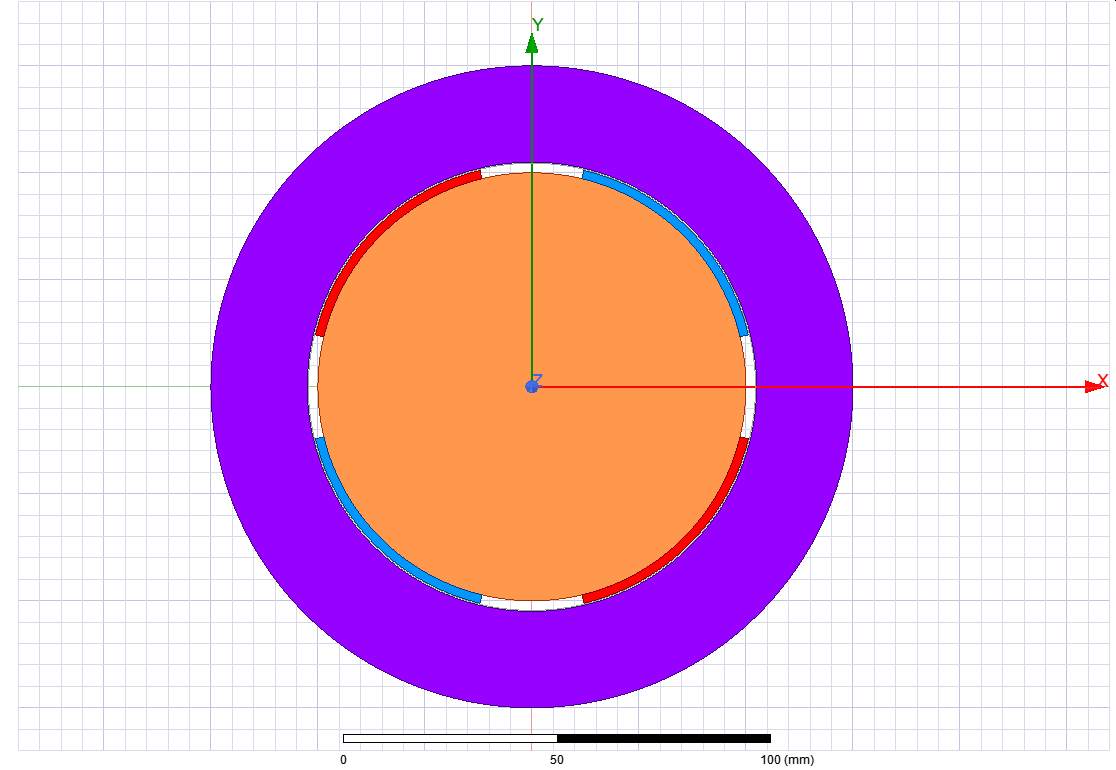
\includegraphics[scale=0.5]{Figures/MachineQ1.png}
\caption{FEA model of the machine for Q1}
\label{fig:MachineQ1}
\end{figure}

\begin{figure}[h!]
\centering
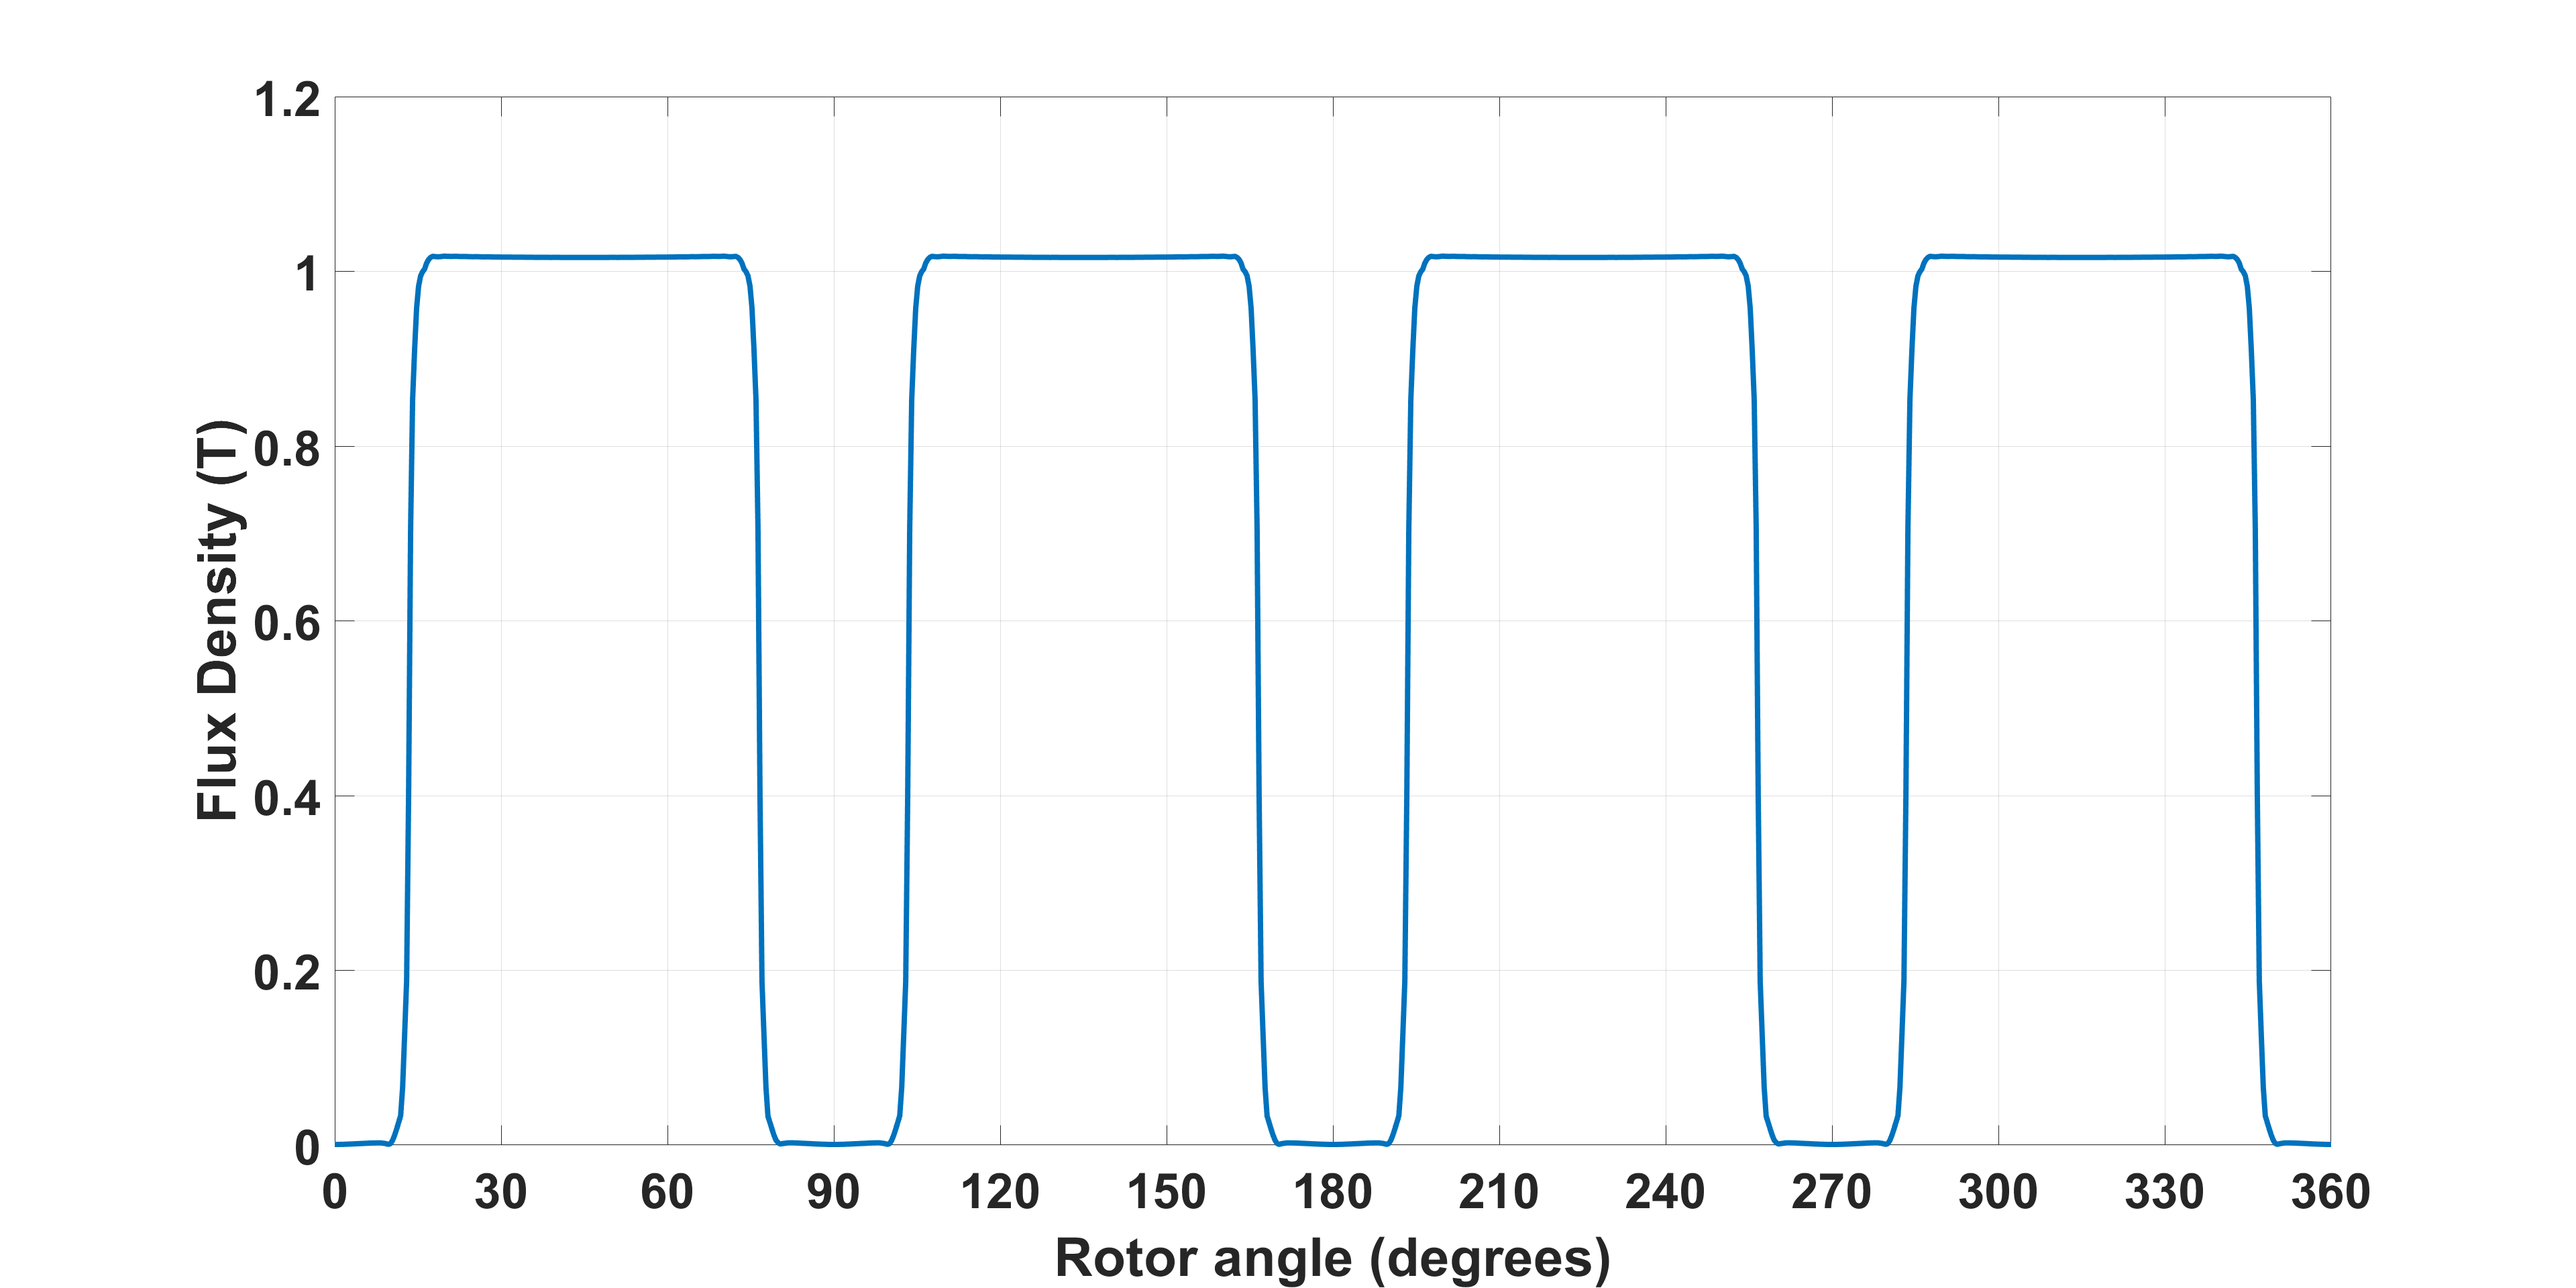
\includegraphics[scale=0.15]{Figures/MagB.png}
\caption{Magnetic Flux Density Magnitude of Figure \ref{fig:MachineQ1}}
\label{fig:MagB}
\end{figure}

\section{Question 2 - Electrical Loading and Machine Sizing}
\subsection{Part - a}
The number of slots are chosen to be 36, which gives out a reasonable slot width value of $4.363 \: \mathrm{mm}$ as calculated in (\ref{eqn:SlotWidth}). Moreover the distribution factors for the chosen number of slots are listed in Table \ref{table:WindingFactor}. The winding factors for the harmonic could be reduced using a different number of slots, which is out of the scope of this study. 



\begin{equation} \label{eqn:SlotWidth}
    W_{Slot} = \frac{\pi \cdot D_i}{2 \cdot N_{slot}} =  4.363 \: \mathrm{mm}
\end{equation}
\begin{table}[h!] 
\begin{center}
\caption{Winding Factors for the chosen slots}
\label{table:WindingFactor}
\begin{tabular}{ |p{3cm}||p{3cm}|p{3cm}|p{3cm}|  }
 \hline
  Harmonic order: & First	& Third &Fifth\\
 \hline
 kd	& $0.96$	&	$0.64$ & $0.192$\\
 \hline
 kp &	$1$	& $-1$	&$1$\\
 \hline
 kw &$0.96$	& $-0.64$&	$0.192$\\
  \hline
 \end{tabular}
 \end{center}
 \end{table}

 \subsection{Part - b}
 For $2.5 \: \mathrm{A_{rms}}$ current and $5 \: \mathrm{\frac{A}{mm^2}}$ current density, the required wire area is calculated in (\ref{eqn:CopperArea}). For the calculated copper wire area, AWG20 cable is chosen whose area and diameter are $0.518 \: \mathrm{mm^2}$ $0.406 \: \mathrm{mm}$ respectively.

\begin{equation} \label{eqn:CopperArea}
    A_{wire} = \frac{2.5 \: \mathrm{A_{rms}}}{5 \: \mathrm{\frac{A}{mm^2}}} =  0.5 \: \mathrm{mm^2}
\end{equation}

\subsection{Part - c}
It is known that the optimal torque value is obtained when slot ratio value is $\frac{1}{\sqrt{3}}$. Therefore, the slot ratio is chosen as $0.6$. Considering the slot ratio, The slot-end diameter and the height of the slots are calculated in (\ref{eqn:SlotHeight}). 

The back core thickness is chosen for a peak flux density value of \textbf{1.5 Tesla}. The resultant stator outer diameter is provided in (\ref{eqn:StatorOuterDiameter}).

\begin{equation} \label{eqn:SlotEndDiameter}
    D_{slotend} = \frac{D_i}{\mathrm{Slot \: Ratio}} = 166.67 \: \mathrm{mm};
\end{equation}
\begin{equation} \label{eqn:SlotHeight}
    H_{slot} = \frac{\mathrm{D_{slotend}-D_i}}{2} = 33.33 \: \mathrm{mm}
\end{equation}
\begin{equation} \label{eqn:BackCoreDepth}
    H_{backcore} = \frac{\phi_{pp}}{\hat{B}_{airgap} \cdot L_{axial}} = 42.6 \: \mathrm{mm}
\end{equation}
\begin{equation} \label{eqn:StatorOuterDiameter}
    D_{o} = \mathrm{D_{slotend}} + 2\cdot H_{backcore}= 251.9 \: \mathrm{mm}
\end{equation}

\subsection{Part - d}
In order to calculate the electrical loading, number of turns per slot must be calculated. To calculate the number of turns, fill factor value is chosen as $\pmb{0.5}$. Note that, the fill factor is chosen relatively low for thermal consideration but may need further iteration. The calculation of the number of turns is provided in (\ref{eqn:NumberOfTurnsPerSlot}).

\begin{equation} \label{eqn:NumberOfTurnsPerSlot}
    N_{turn} = \frac{H_{slot} \cdot W_{slot} \cdot FillFactor}{A_{AWG20}} \approx 141 \: \frac{\mathrm{turns}}{\mathrm{slot}}
\end{equation}


The electrical loading of the machine is provided in (\ref{eqn:ElectricalLoading}). The current value was stated as $2.5 \: A_{rms}$. 
\begin{equation} \label{eqn:ElectricalLoading}
    A_{rms} = \frac{N_{turn} \cdot I_{rms} \cdot N_{slot}}{\pi \cdot \: D_i} = 40393.52 \: \mathrm{\frac{\mathrm{A}}{\mathrm{m}}}
\end{equation}



The obtained $40.4 \frac{\mathrm{kA}}{m}$ value is in the reasonable range which is between $35-65 \frac{\mathrm{kA}}{\mathrm{m}}$.

\subsection{Part - e}
The peak airgap flux density is found as $1.0174\: \mathrm{T} $ from the FEA results. The resultant average tangential stress and total force are provided in (\ref{eqn:AverageStress}) and (\ref{eqn:TotalForce}) respectively.
\begin{equation} \label{eqn:AverageStress}
    \sigma_{tan} = \frac{A_{rms} \cdot \hat{B} \cdot cos(\phi)}{\sqrt{2}} = 29059.81 \: \mathrm{Pa}
\end{equation}
\begin{equation} \label{eqn:TotalForce}
    F = \sigma_{tan} \cdot \pi \cdot D_i \cdot L_{axial} = 912.94 \: \mathrm{Newton}
\end{equation}
\begin{equation} \label{eqn:Torque}
    T = \frac{F \cdot D_i}{2} = 45.65 \: \mathrm{Nm}
\end{equation}

\subsection{Part - f}
At a rated speed of 1500 rpm, the power of the machine can be calculated in (\ref{eqn:Power}).

\begin{equation} \label{eqn:Power}
    P = T \cdot \omega  = 7.17 \: \mathrm{kW}
\end{equation}


\section{Question 3 - Comparison and Optimization }
\subsection{Part - a}
In this section, the machine outer diameter is fixed and other parameters can be modified. In order to increase overall flux and preventing saturation, the \textbf{magnet to pole pitch ratio} is increased to 1. 

With a fixed outher diameter of $160$ \: mm , the inner diameter end the slot end diameter needs to be chosen first. It has been stated that optimum $\frac{\mathrm{Rotor diameter}}{\mathrm{Slot end diameter}}$ is around 0.6. We need to have a relation between the stator outer diameter and the rotor diameter, which is shown in equations (\ref{eqn:StatorOuterDiameterNew})(\ref{eqn:BackCoreDepthNew})(\ref{eqn:FluxPerPoleNew})(\ref{eqn:MagnetAreaPerPoleNew})(\ref{eqn:PoleAreaNew}). This way, the rotor diameter can be related to the stator outer diameter.

\begin{equation} \label{eqn:StatorOuterDiameterNew}
    D_{o} = \mathrm{D_{i}} + 2\cdot H_{backcore}
\end{equation}
\begin{equation} \label{eqn:BackCoreDepthNew}
    H_{backcore} = \frac{\hat{\phi_{pp}}}{\hat{B}_{backcore} \cdot L_{axial}} 
\end{equation}
\begin{equation} \label{eqn:FluxPerPoleNew}
    \hat{\phi_{pp}} = A_{magnetperpole}\cdot \hat{B}_{airgap}
\end{equation}
\begin{equation} \label{eqn:MagnetAreaPerPoleNew}
    A_{magnetperpole} = A_{pole} 
\end{equation}
\begin{equation} \label{eqn:PoleAreaNew}
    A_{pole} = \frac{\pi \: D_i \: L_{axial}}{N_{pole}}
\end{equation}

After combining, a cofficient that relates the outer diameter to rotor diameter is obtained in (\ref{eqn:RotorDiameterCoefficient}).

\begin{equation} \label{eqn:RotorDiameterCoefficient}
    D_{i-coefficient} = \frac{1}{\mathrm{Slot \: Ratio}} + (\frac{\pi \cdot L_{axial}}{N_{pole}})\cdot \mathrm{MagnetToPolePitchRatio} \cdot \hat{B_{airgap}}\cdot \frac{1}{\hat{B_{backcore}}\cdot L_{axial}}\cdot 2 = 2.45
\end{equation}

\begin{equation} \label{eqn:RotorDiameterNew}
    D_{i} = \frac{D_o}{D_{i-coefficient}} = 65.25 \: \mathrm{mm}
\end{equation}
\begin{equation} \label{eqn:SlotEndDiameterNew}
    D_{slotend} = \frac{D_i}{\mathrm{Slot \: Ratio}} = 108.75 \: \mathrm{mm};
\end{equation}


Note that the air gap flux density is reduced to \textbf{0.75 Tesla} in order not to cause saturation on the teeth. After finding the rotor diameter, the overall flux density is reduced by decreasing the height of the magnets, as shown in (\ref{eqn:MagnetAreaPerPoleNewNew}),(\ref{eqn:NonMagnetAreaPerPoleNew}),(\ref{eqn:MagnetReluctanceNew}),(\ref{eqn:AirGapReluctanceNew}),(\ref{eqn:MmfPerMagnetNew}),(\ref{eqn:AirGapFluxNew}),(\ref{eqn:AirGapFluxDensityNew}) (the obtained result in (\ref{eqn:AirGapFluxDensityNew}) is for 0.8 T, there is a margin for the leakage flux).

\begin{equation} \label{eqn:MagnetAreaPerPoleNewNew}
    A_{magnetperpole} = A_{pole} = 0.005125 \: \mathrm{m^2}
\end{equation}

\begin{equation} \label{eqn:NonMagnetAreaPerPoleNew}
    A_{nonmagnetperpole} = 0
\end{equation}

\begin{equation} \label{eqn:MagnetReluctanceNew}
    R_{m1}  =  R_{m2} =  \frac{H_{magnet}}{A_{magnetperpole} \cdot \mu_0 \cdot \mu_r}  = 236615 \: \mathrm{\frac{1}{Henry}} 
\end{equation}

\begin{equation} \label{eqn:AirGapReluctanceNew}
    R_{ag1}  =  R_{ag2} =  \frac{H_{airgap}}{A_{magnetperpole} \cdot \mu_0}  =  155278  \: \mathrm{\frac{1}{Henry}} 
\end{equation}

\begin{equation} \label{eqn:MmfPerMagnetNew}
    \mathcal{F}_{permagnet} = A_{magnetperpole} \cdot B_{residual} \cdot R_{m1} = 1600 \: \mathrm{Amperes}
\end{equation}

\begin{equation} \label{eqn:AirGapFluxNew}
    \phi_{m} = \frac{2 \cdot \mathcal{F}_{permagnet}}{R_{m1}+R_{m2}+R_{ag1}+R_{ag2}} = 4.084 \: \mathrm{mWeber}
\end{equation}

\begin{equation} \label{eqn:AirGapFluxDensityNew}
    B_{m} = \frac{\phi_{m}}{A_{magnetperpole}} = 0.7970 \: \mathrm{Tesla}
\end{equation}

The backcore depth is provided in (\ref{eqn:BackCoreDepthNewNew}).
\begin{equation} \label{eqn:BackCoreDepthNewNew}
    H_{backcore} = \frac{D_o - D_{slotend}}{2} = 25.6 \: \mathrm{mm}
\end{equation}

For the same current value and the new slot area values, the number of turns required is given in (\ref{eqn:NumberOfTurnsPerSlotNew}).

\begin{equation} \label{eqn:NumberOfTurnsPerSlotNew}
    N_{turn} = \frac{H_{slot} \cdot W_{slot} \cdot FillFactor}{A_{AWG20}} \approx 122 \: \frac{\mathrm{turns}}{\mathrm{slot}}
\end{equation}

\begin{equation} \label{eqn:MagneticLoadingNew}
    \bar{B} = \frac{N_{pole}\:\phi_{m}}{\pi \: D_i \: L_{axial}} = 0.7970 \: \mathrm{Tesla}
\end{equation}

\begin{equation} \label{eqn:ElectricalLoadingNew}
    A_{rms} = \frac{N_{turn} \cdot I_{rms} \cdot N_{slot}}{\pi \cdot \: D_i} = 53563 \: \mathrm{\frac{\mathrm{A}}{\mathrm{m}}}
\end{equation}

\begin{equation} \label{eqn:AverageStressNew}
    \sigma_{tan} = \frac{A_{rms} \cdot \hat{B} \cdot cos(\phi)}{\sqrt{2}} = 28406 \: \mathrm{Pa}
\end{equation}
\begin{equation} \label{eqn:TotalForceNew}
    F = \sigma_{tan} \cdot \pi \cdot D_i \cdot L_{axial} = 582.3 \: \mathrm{Newton}
\end{equation}
\begin{equation} \label{eqn:TorqueNew}
    T = \frac{F \cdot D_i}{2} = 19 \: \mathrm{Nm}
\end{equation}

\begin{equation} \label{eqn:PowerNew}
    P = T \cdot \omega  \approx 2.98 \: \mathrm{kW}
\end{equation}

Looking at the machine designed in this part, comparison of the machines are provided in Table \ref{table:Comparison}. 
Moreover, the magnetostatic analysis of the airgap flux density is provided in Fig.\ref{fig:MagBQ3}. Due to the teeth opening, the airgap flux density varies between 0.82T to 0.53T. The mean airgap flux density is calculated to be around \textbf{0.7T}.
\begin{figure}[h!]
\centering
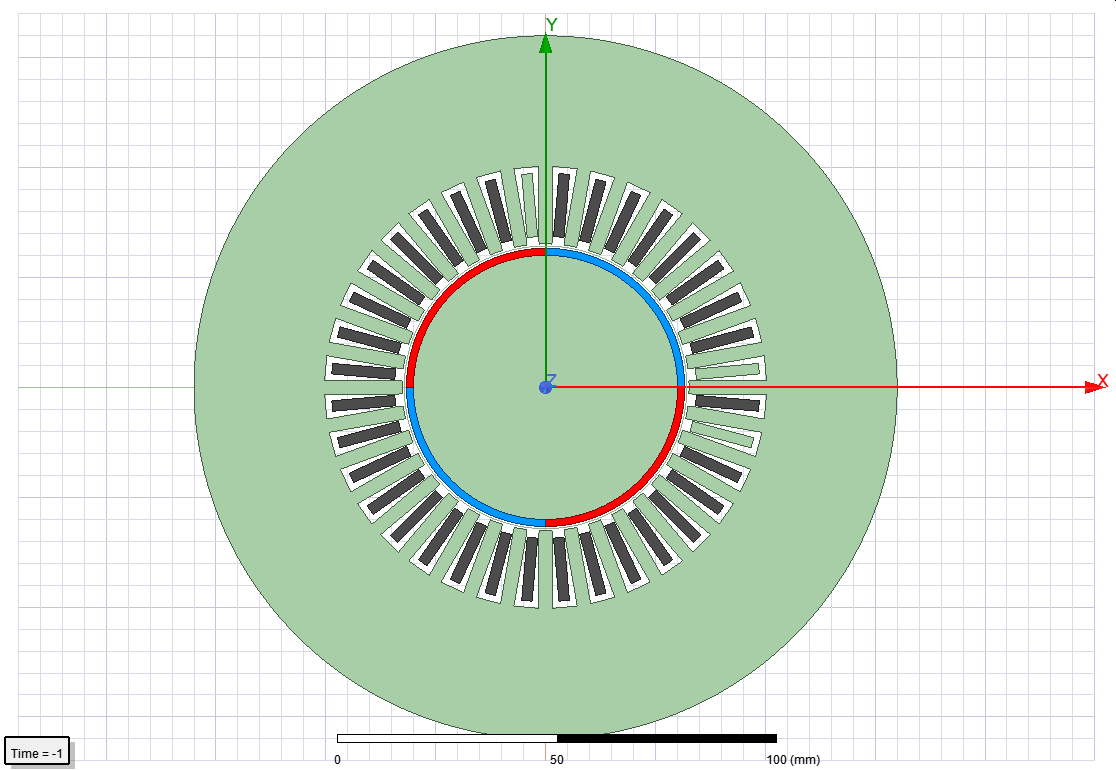
\includegraphics[scale=0.5]{Figures/MachineQ3.png}
\caption{FEA model of the machine for Q3-a}
\label{fig:MachineQ3}
\end{figure}

\begin{figure}[h!]
\centering
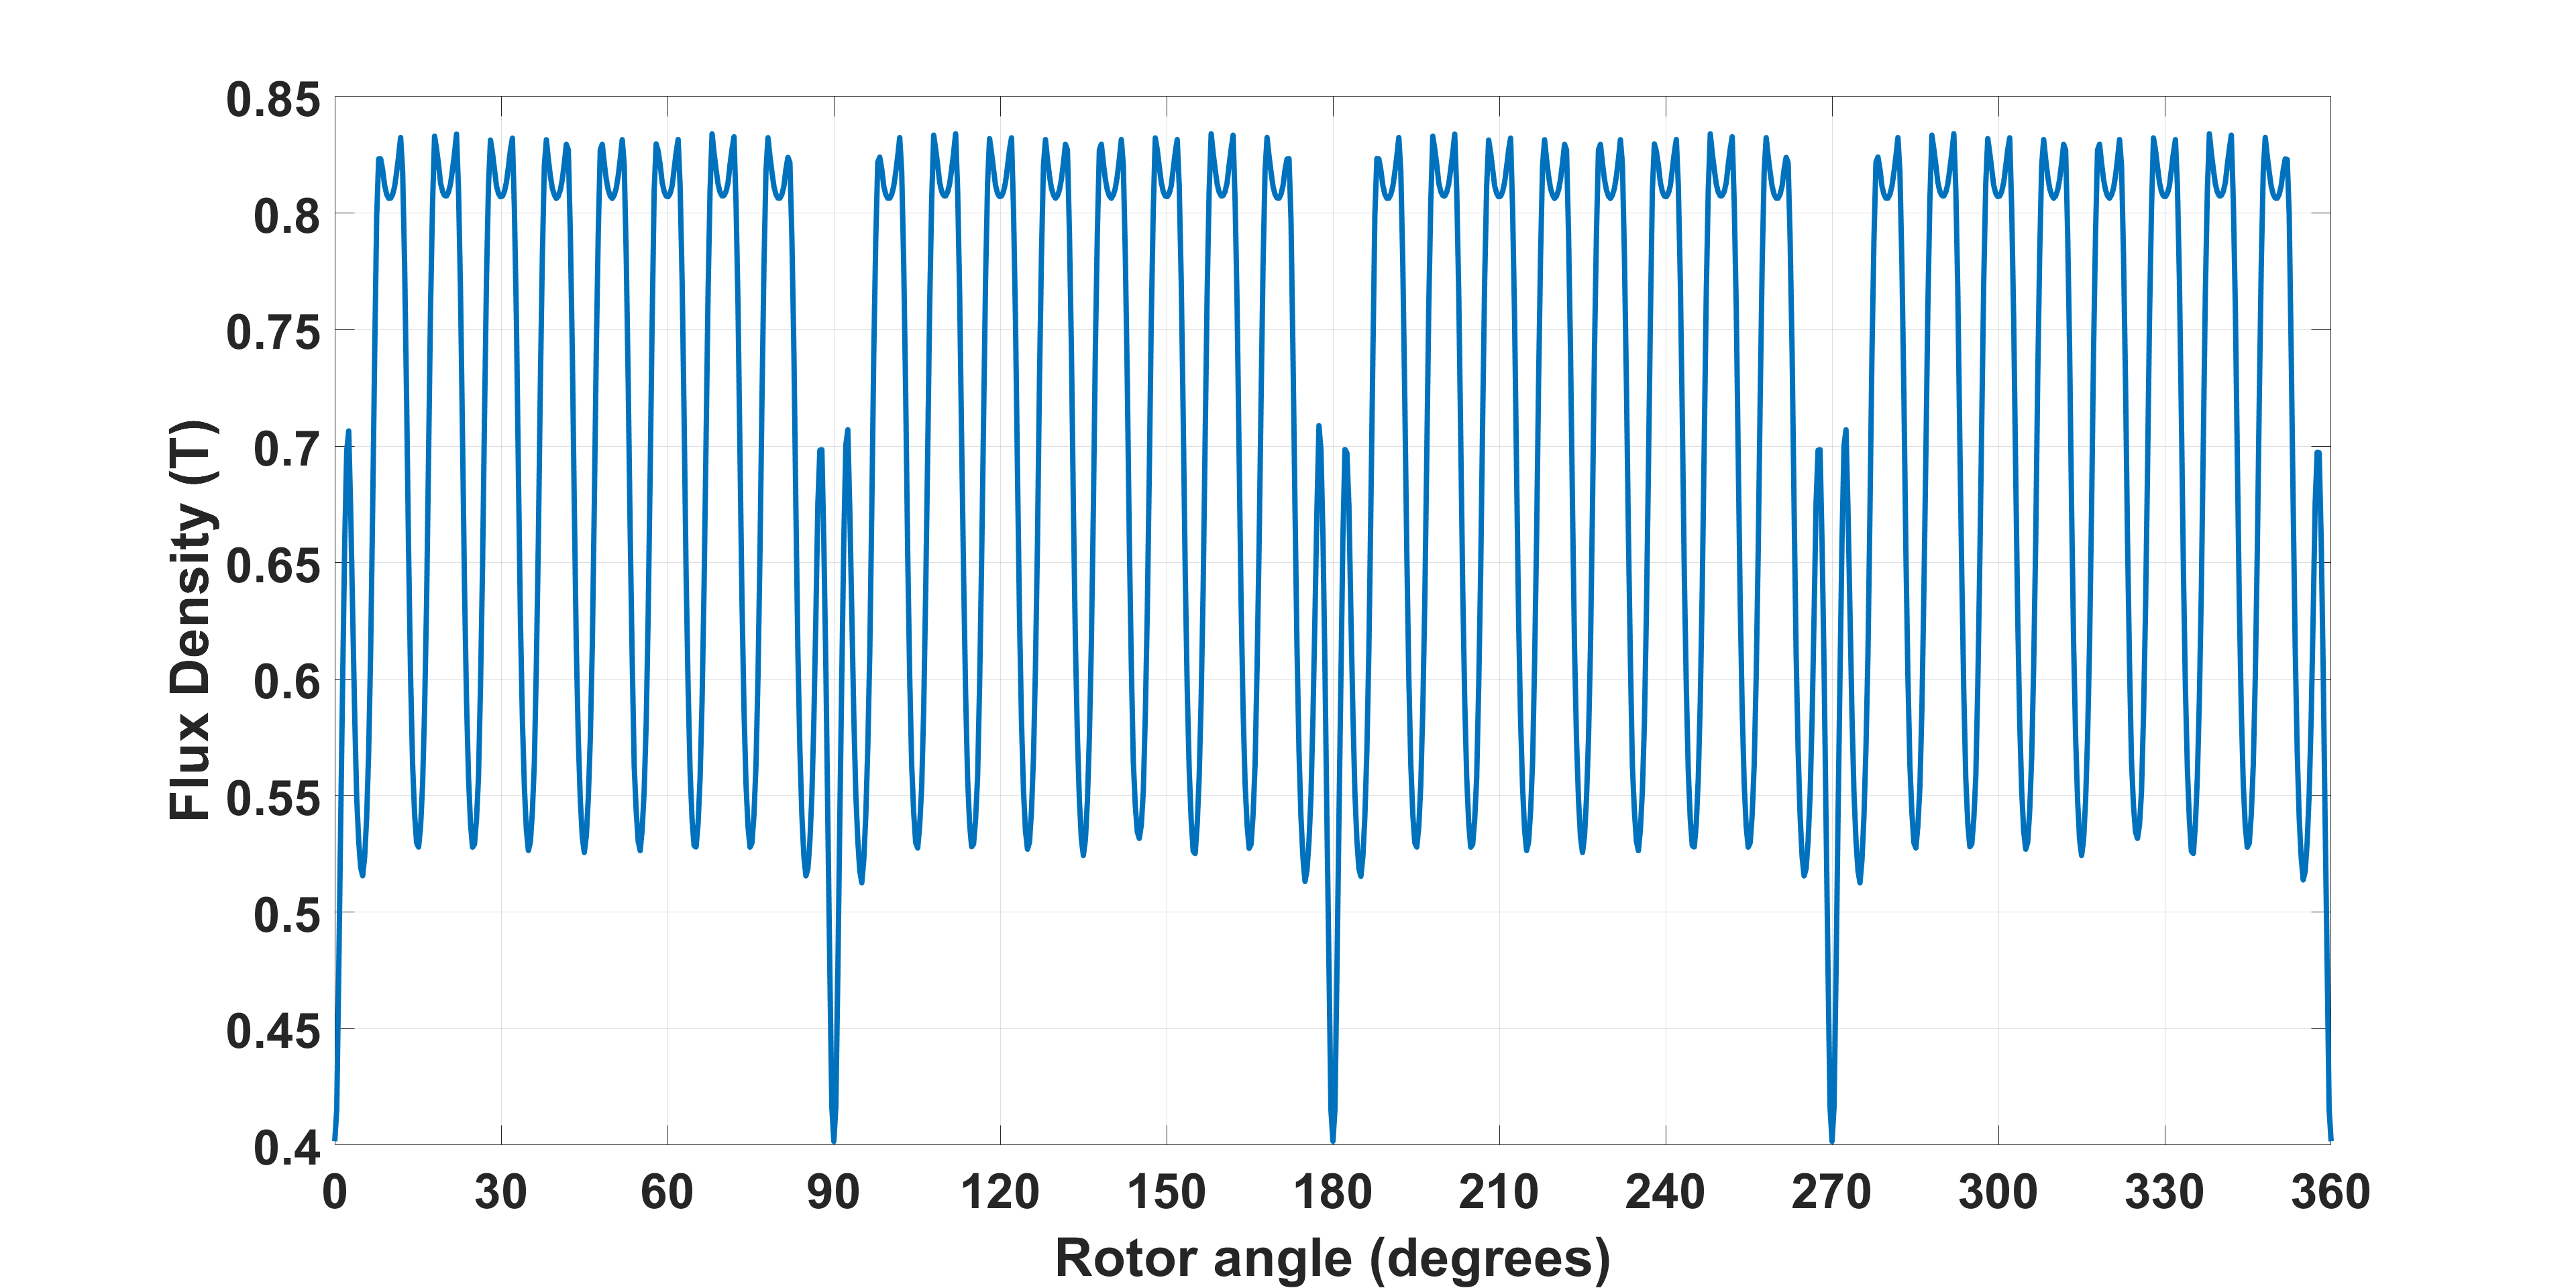
\includegraphics[scale=0.15]{Figures/MagBQ3.png}
\caption{Magnetic Flux Density Magnitude for Figure \ref{fig:MachineQ3}}
\label{fig:MagBQ3}
\end{figure}

\begin{table}[h!] 
\begin{center}
\caption{Machine parameter comparison for the optimized and unoptimized neodymium machines}
\label{table:Comparison}
\begin{tabular}{ |p{3cm}||p{3cm}|p{3cm}|p{3cm}|  }
 \hline
    & Q1-Q2	& Q3-a\\
 \hline
 $D_i$	& $100mm$	&	$65.3mm$\\
 \hline
 $D_o$ &	$251.9mm$	& $160mm$\\
 \hline
 $D_{slotend}$ &$166.67mm$	& $108.8mm$\\
 \hline
  $Torque$ &$45.65Nm$	& $19Nm$\\
 \hline
  $Power$ &$7.17kW$	& $2.98kW$\\
 \hline
  $Size$ &$0.005m^3$	& $0.002m^3$\\
 \hline
\end{tabular}
\end{center}
\end{table}

\subsection{Part - b}
After changing the permanent magnet to ferrite, the overall flux density decreased to its $\frac{0.4}{1.32}$. This changes the magnetic loading of the machine as represented in (\ref{eqn:MagneticLoadingNewNew}). 

\begin{equation} \label{eqn:MagneticLoadingNewNew}
    \bar{B} = \frac{N_{pole}\:\phi_{m}}{\pi \: D_i \: L_{axial}} = 0.3168 \: \mathrm{Tesla}
\end{equation}

The new magnetic loading value will result in a reduction of tangential stress of the machine. The updated machine parameters are as follows.

\begin{equation} \label{eqn:AverageStressNewNew}
    \sigma_{tan} = \frac{A_{rms} \cdot \hat{B} \cdot cos(\phi)}{\sqrt{2}} = 8608 \: \mathrm{Pa}
\end{equation}
\begin{equation} \label{eqn:TotalForceNewNew}
    F = \sigma_{tan} \cdot \pi \cdot D_i \cdot L_{axial} = 176.45 \: \mathrm{Newton}
\end{equation}
\begin{equation} \label{eqn:TorqueNewNew}
    T = \frac{F \cdot D_i}{2} = 5.75 \: \mathrm{Nm}
\end{equation}

\begin{equation} \label{eqn:PowerNewNew}
    P = T \cdot \omega  \approx 904 \: \mathrm{W}
\end{equation}

It can be seen that the machine performance is directly affected by the permanent magnet change. Since the overall flux inside the airgap of the machine is reduced, the torque generated by the magnets will be reduced, which will degrade the machine's performance. If more torque is needed, thicker ferrite magnets may be used to increase airgap flux.



\subsection{Part - c}
By following the same procedure presented in Question 3-a, the optimum point for the ferrite machine has been chosen. The corresponding machine parameters with unoptimized and optimized ferrite machine is provided in Table \ref{table:ComparisonFerrite}. 

Other parameters of this machine can be listed as:
\begin{itemize}
    \item Magnet thickness: 4mm
    \item $\hat{B}_{airgap}$: 0.3 Tesla
    \item Backcore length 16.1mm
    \item Slot area 1.81e-4 $m^2$
    \item $N_{turn}$: 176 $\frac{turns}{slot}$
\end{itemize}

Since the ferrite machines have lower residual flux density, it has lower torque and power rating for the same volume. 
The neodymium magnet machine has 122 turns per slot while the ferrite machine has 198 turns per slot. This means that the copper cost of the ferrite machine will be higher. 
On the other hand, since unit price for neodymium magnets are higher, the ferrite magnets will have a lower cost.


\begin{table}[h!] 
\begin{center}
\caption{Machine parameter comparison for the optimized and unoptimized ferrite machines}
\label{table:ComparisonFerrite}
\begin{tabular}{ |p{3cm}||p{3cm}|p{3cm}|p{3cm}|  }
 \hline
   & Q3-b	& Q3-c\\
 \hline
 $D_i$	& $65.3mm$	&	$80.8mm$\\
 \hline
 $D_o$ &	$160mm$	& $160mm$\\
 \hline
 $D_{slotend}$ &$108.8 mm$	& $134.6mm$\\
 \hline
  $Torque$ &$5.75Nm$	& $15.6Nm$\\
 \hline
  $Power$ &$904W$	& $2.4kW$\\
 \hline
\end{tabular}
\end{center}
\end{table}




% \begin{equation} \label{eqn:CopperRadius}
%    R_{copper} = \sqrt{\frac{A_{wire}}{\pi}} =  0.5 \: \mathrm{mm^2}
%\end{equation}
%
%
% Memoization
\bibliographystyle{plain}
\end{document}